%----------------------------------------------------------------------
%----------------------------------------------------------------------
\section{Success Stories}
\begin{frame}[c]{Success Stories}
\framesubtitle{HPO in the real world}
\begin{itemize}
    \item Spearmint
    \item Hyperopt and Hyperopt-SKLearn
    \item Auto-sklearn
\end{itemize}

\end{frame}
%-----------------------------------------------------------------------
\begin{frame}[c]{Spearmint}
\pause
\begin{center}
    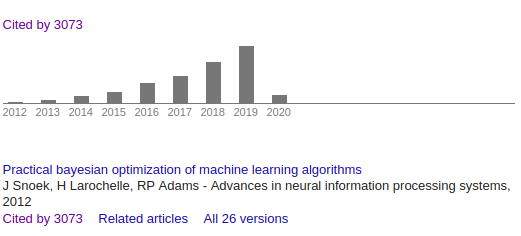
\includegraphics[width=.9\linewidth, height=0.9\textheight, keepaspectratio=true]{w07_hpo_grey_box/images/success_stories/spearmint_alt_stats.png}
    \newline \paragraph{Google Scholar screenshot from 3rd March, 2020}
\end{center}
\end{frame}
%-----------------------------------------------------------------------
\begin{frame}[c]{Spearmint}
\pause
\begin{itemize}
    \item<+-> One of the first available comprehensive packages for performing HPO with state-of-the-art results at the time on deep neural networks.
    
    \item<+-> Open-source and non-commercial license based implementation available on Github.
    
    \item<+-> TODO: Include reference to state-of-the-art of Spearmint
\end{itemize}

\begin{center}
    \only<+->{
\includegraphics[width=\linewidth, height=\textheight, keepaspectratio=true]{w07_hpo_grey_box/images/success_stories/jsnoek_spearmint_git_stats.png}}
    
    \only<+->{
\includegraphics[width=\linewidth, height=\textheight, keepaspectratio=true]{w07_hpo_grey_box/images/success_stories/hips_spearmint_git_stats.png}}
\end{center}
\end{frame}

%-----------------------------------------------------------------------

\begin{frame}[c]{Hyperopt and Hyperopt-SKLearn}
\pause
\begin{itemize}
    \item<+-> Hyperopt is a python package for performing HPO over a user-described search space of parameters.
    \item<+-> Hyperopt-SKLearn is a software project that uses Hyperopt to automate the optimization of the SciKit-Learn library.
    \item<+-> TODO: Include stuff from the TPE paper "Making a Science of Model Search" http://proceedings.mlr.press/v28/bergstra13.pdf
\end{itemize}

\begin{center}
    \only<+->{
\includegraphics[width=\linewidth, height=\textheight, keepaspectratio=true]{w07_hpo_grey_box/images/success_stories/hyperopt_git_stats.png}}
    
    \only<+->{
\includegraphics[width=\linewidth, height=\textheight, keepaspectratio=true]{w07_hpo_grey_box/images/success_stories/hyperopt_sklearn_git_stats.png}}
\end{center}
\end{frame}

%-----------------------------------------------------------------------

\begin{frame}[c]{Auto-sklearn}
\pause
\begin{itemize}
    \item<+-> TODO: Include usage statistics, salient features, references
\end{itemize}
\end{frame}

%-----------------------------------------------------------------------

\begin{frame}[c]{AlphaGo}
\pause
\begin{itemize}
    \item<+-> TODO: AlphaGo used BO repeatedly during its lifecycle
    \item<+-> TOOD: Find and reference paper
    \item<+-> TODO: Quote figures from the paper
\end{itemize}
\end{frame}

%-----------------------------------------------------------------------